\documentclass[tikz,border=8pt]{standalone}
\usepackage[T1]{fontenc}
\usepackage{times}
\usetikzlibrary{positioning,arrows.meta,fit,backgrounds,calc,shapes.geometric}
\definecolor{structC}{HTML}{4C72B0}
\definecolor{obsC}{HTML}{5A9E6F}
\definecolor{hypC}{HTML}{DD8452}
\definecolor{guideC}{HTML}{8E6BB0}
\definecolor{evidC}{HTML}{B0544C}
\definecolor{darkC}{HTML}{343434}
\begin{document}
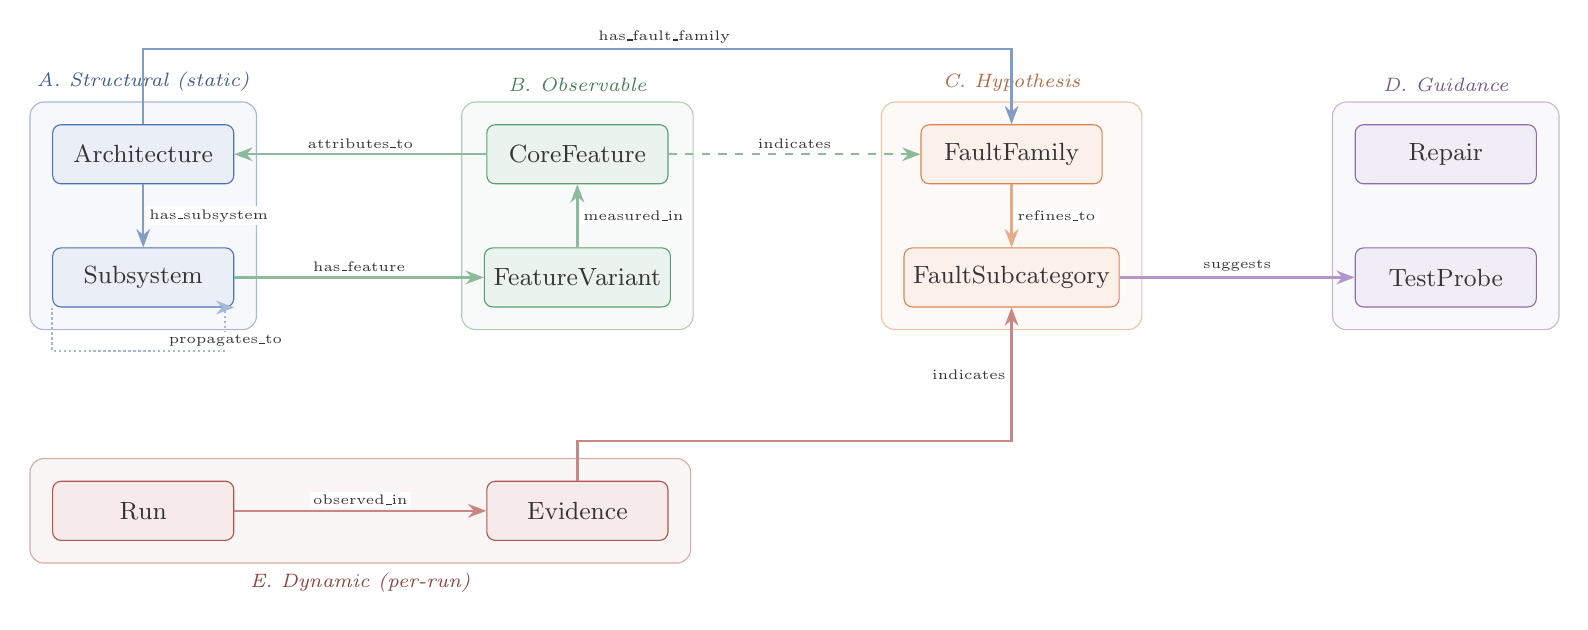
\begin{tikzpicture}[
  >=Stealth,
  every node/.style={font=\rmfamily\small, text=darkC},
  typebox/.style={draw=#1, fill=#1!12, rounded corners=3pt,
                  minimum width=2.3cm, minimum height=0.75cm,
                  font=\rmfamily\small, text=darkC, align=center},
  edgelbl/.style={font=\rmfamily\tiny, text=darkC, fill=white,
                  inner sep=1.2pt, outer sep=1pt},
  catbox/.style={draw=#1!50, fill=#1!5, rounded corners=5pt,
                 inner sep=8pt},
]

% ── Column 1: Structural ──
\node[typebox=structC] (arch) {Architecture};
\node[typebox=structC, below=0.8 of arch] (subsys) {Subsystem};

% ── Column 2: Observable ──
\node[typebox=obsC, right=3.2 of arch] (core) {CoreFeature};
\node[typebox=obsC, below=0.8 of core] (fvar) {FeatureVariant};

% ── Column 3: Hypothesis ──
\node[typebox=hypC, right=3.2 of core] (fam) {FaultFamily};
\node[typebox=hypC, below=0.8 of fam] (sub) {FaultSubcategory};

% ── Column 4: Guidance ──
\node[typebox=guideC, right=3.2 of fam] (rem) {Repair};
\node[typebox=guideC, below=0.8 of rem] (probe) {TestProbe};

% ── Row 3: Dynamic ──
\node[typebox=evidC, below=2.2 of subsys] (run) {Run};
\node[typebox=evidC, right=3.2 of run] (evid) {Evidence};

% ── Category backgrounds ──
\begin{scope}[on background layer]
  \node[catbox=structC, fit=(arch)(subsys), label={[font=\rmfamily\scriptsize\itshape,
        text=structC!80!black]above:A.~Structural (static)}] {};
  \node[catbox=obsC, fit=(core)(fvar), label={[font=\rmfamily\scriptsize\itshape,
        text=obsC!80!black]above:B.~Observable}] {};
  \node[catbox=hypC, fit=(fam)(sub), label={[font=\rmfamily\scriptsize\itshape,
        text=hypC!80!black]above:C.~Hypothesis}] {};
  \node[catbox=guideC, fit=(rem)(probe), label={[font=\rmfamily\scriptsize\itshape,
        text=guideC!80!black]above:D.~Guidance}] {};
  \node[catbox=evidC, fit=(run)(evid), label={[font=\rmfamily\scriptsize\itshape,
        text=evidC!80!black]below:E.~Dynamic (per-run)}] {};
\end{scope}

% ── Edge: has_subsystem (A down) ──
\draw[->, thick, structC!70]
  (arch) -- node[edgelbl, right]{has\_subsystem} (subsys);

% ── Edge: has_fault_family (A -> C, routed well above category labels) ──
\draw[->, thick, structC!70]
  (arch.north) -- ++(0,0.95) -| node[edgelbl, above, pos=0.3]{has\_fault\_family} (fam.north);

% ── Edge: measured_in (B up) ──
\draw[->, thick, obsC!70]
  (fvar) -- node[edgelbl, right]{measured\_in} (core);

% ── Edge: attributes_to (B -> A) ──
\draw[->, thick, obsC!70]
  (core.west) -- node[edgelbl, above]{attributes\_to} (arch.east);

% ── Edge: has_feature (A -> B) ──
\draw[->, thick, obsC!70]
  (subsys.east) -- node[edgelbl, above]{has\_feature} (fvar.west);

% ── Edge: refines_to (C down) ──
\draw[->, thick, hypC!70]
  (fam) -- node[edgelbl, right]{refines\_to} (sub);

% ── Edge: suggests (C -> D) ──
\draw[->, thick, guideC!70]
  (sub.east) -- node[edgelbl, above]{suggests} (probe.west);

% ── Edge: indicates (B -> C, dashed) ──
\draw[->, thick, obsC!70, dashed]
  (core.east) -- node[edgelbl, above]{indicates} (fam.west);

% ── Edge: indicates (E -> C) ──
\draw[->, thick, evidC!70]
  (evid.north) -- ++(0,0.5) -| node[edgelbl, left, pos=0.75]{indicates} (sub.south);

% ── Edge: observed_in (E) ──
\draw[->, thick, evidC!70]
  (run.east) -- node[edgelbl, above]{observed\_in} (evid.west);

% ── Edge: propagates_to (self-loop on Subsystem) ──
\draw[->, thick, structC!50, densely dotted]
  (subsys.south west) -- ++(0,-0.55) -- ++(2.2,0) -- ++(0,0.55)
  node[edgelbl, below, pos=0.5]{propagates\_to} -- (subsys.south east);

\end{tikzpicture}
\end{document}
